\documentclass{theme}


\misc{Homomorphic Encryption via Ring Learning With Errors (RLWE)}
\due{May 12th, 2024}

\usepackage{titlesec}
\titlespacing*{\section}{0pt}{0.2\baselineskip}{0.2\baselineskip}
\titlespacing*{\subsection}{0pt}{0.15\baselineskip}{0.15\baselineskip}
\titlespacing*{\subsubsection}{0pt}{0.1\baselineskip}{0.1\baselineskip}

\usepackage[outputdir=../../]{minted}

\course{MATH 1580 - Spring 2024}{Cryptography}{Professor Vogt}

% Add bibliography
\usepackage[backend=biber]{biblatex}
\addbibresource{references.bib}

%Packages
\usepackage{geometry}
\usepackage{amsmath}
\usepackage{amsfonts}
\usepackage{mathtools}
\usepackage{amsthm}
\usepackage{mhchem}
\usepackage{multicol}
\usepackage{gensymb}
\usepackage{chemfig}
\usepackage{tikz}
\usepackage{pgfplots}
\usepackage{listings}
\usepackage{xcolor}
\usepackage{hyperref}
\usepackage{booktabs}
\usepackage{pgfplotstable}
\usepackage{graphicx}
\usepackage{caption}
\usepackage{commath}
\usepackage{centernot}
\usepackage{tikz-cd}
\usepackage{enumitem}
\usepackage{cryptocode}
\usepackage{amssymb}
\usepackage[shortlabels]{enumitem}
\hypersetup{
  colorlinks,
  citecolor=black,
  filecolor=black,
  linkcolor=black,
  urlcolor=black
}
\graphicspath{ {./images/} }
%Custom Environments

%A generic custom theorem header
\newtheoremstyle{ntheoremstyle}% name of the style to be used
{}% measure of space to leave above the theorem. E.g.: 3pt
{}% measure of space to leave below the theorem. E.g.: 3pt
{\it}% name of font to use in the body of the theorem
{}% measure of space to indent
{\bfseries}% name of head font
{}% punctuation between head and body
{ }% space after theorem head; " " = normal interword space
{\thmname{#3}.}
\theoremstyle{ntheoremstyle}
\newtheorem{ntheorem}{Theorem}[section]

\newtheoremstyle{ndefinitionstyle}% name of the style to be used
{}% measure of space to leave above the theorem. E.g.: 3pt
{}% measure of space to leave below the theorem. E.g.: 3pt
{}% name of font to use in the body of the theorem
{}% measure of space to indent
{\bfseries}% name of head font
{}% punctuation between head and body
{ }% space after theorem head; " " = normal interword space
{\thmname{#3}.}
\theoremstyle{ndefinitionstyle}
\newtheorem{ndefinition}{Theorem}[section]

\newtheoremstyle{nproofstyle}% name of the style to be used
{}% measure of space to leave above the theorem. E.g.: 3pt
{}% measure of space to leave below the theorem. E.g.: 3pt
{}% name of font to use in the body of the theorem
{}% measure of space to indent
{\bfseries}% name of head font
{}% punctuation between head and body
{ }% space after theorem head; " " = normal interword space
{\thmname{#3}.}
\theoremstyle{nproofstyle}
\newtheorem{nproof}{Proof}[section]
%Custom Commands
\newcommand{\ringmod}[1]{$\mathbb{Z}$/#1$\mathbb{Z}$}
\newcommand{\Z}{\mathbb{Z}}
\newcommand{\R}{\mathbb{R}}
\newcommand{\N}{\mathbb{N}}
\newcommand{\C}{\mathbb{C}}
\newcommand{\F}{\mathbb{F}}
\newcommand{\Q}{\mathbb{Q}}
\newcommand{\Eu}{\mathbb{E}}
\newcommand{\PGL}{\text{PGL}}
\newcommand{\GL}{\text{GL}}
\newcommand{\Aut}{\text{Aut}}
\newcommand{\Endo}{\text{End}}
\newcommand{\E}[1]{\mathbb{E}\left[ #1 \right]}
\newcommand{\Mod}[1]{\ (\mathrm{mod}\ #1)}
\newcommand{\subproblem}[2]{\noindent \ \ \ \ \ \ \ \ \ \ (#1) \ \ #2 \newline\noindent}
\newcommand{\Lim}{\lim\limits}
\newcommand{\Int}{\displaystyle \int}
\newcommand{\Equation}[2]{\begin{equation}
    #2 \tag{#1} \label{eq: #1}
  \end{equation}}
\newcommand{\trace}{\text{trace} \ }
\newcommand{\Var}{\text{Var}}
\newcommand{\Tor}{\text{Tor}}
\newcommand{\cross}{\times}
\newcommand{\vmat}[1]{\begin{vmatrix} #1 \end{vmatrix}}
\newcommand{\bmat}[1]{\begin{bmatrix} #1 \end{bmatrix}}
\newcommand{\pmat}[1]{\begin{pmatrix} #1 \end{pmatrix}}
\newcommand{\eqq}{\stackrel{?}{=}}
\newcommand{\p}[1]{\left( #1 \right)}
\DeclarePairedDelimiter\floor{\lfloor}{\rfloor}
\DeclarePairedDelimiter\ceil{\lceil}{\rceil}
\DeclarePairedDelimiter\babs{\bigg \lvert}{\bigg \rvert}
\newcommand{\note}[1]{\begin{changemargin}{.5cm}{.5cm}\emph{\underline{Note}:} #1 \end{changemargin}}
\def\changemargin#1#2{\list{}{\rightmargin#2\leftmargin#1}\item[]}
\let\endchangemargin=\endlist
\newcommand{\xor}{\ \underline{\lor} \ }
\newcommand{\suchthat}{\ \text{s.t.} \ }
\newcommand{\spanof}{\text{span} \ }
\newcommand{\code}[1]{\lstinline{#1}}
\DeclareMathOperator*{\argmax}{arg\,max}
\DeclareMathOperator*{\argmin}{arg\,min}
\newcommand{\tr}{\text{tr} \ }
\newcommand{\sign}{\text{sign}}
\newcommand{\mc}[1]{\mathcal{#1}}
%Crypto Stuff
\newcommand{\sendright}[1]{\sendmessageright{top=\text{#1}}}
\newcommand{\sendleft}[1]{\sendmessageleft{top=\text{#1}}}

%Chem Stuff
\newcommand{\aq}{_{(aq)}}

\newcommand{\rarrow}{$\to$ }
\newcommand{\imp}{$\implies$}
%Physics
\newcommand{\ihat}{\hat{i}}
\newcommand{\jhat}{\hat{j}}
\newcommand{\khat}{\hat{k}}
\newcommand{\avg}{\text{avg}}
\usepackage{mathtools}
\DeclarePairedDelimiter\bra{\langle}{\rvert}
\DeclarePairedDelimiter\bk{\langle}{\rangle}
\DeclarePairedDelimiter\ket{\lvert}{\rangle}
\DeclarePairedDelimiterX\braket[2]{\langle}{\rangle}{#1 \delimsize\vert #2}
%Units
\newcommand{\m}{\text{m}}
\newcommand{\nm}{\text{nm}}
\newcommand{\s}{\text{s}}
\newcommand{\kg}{\text{kg}}
\newcommand{\ft}{\text{ft}}
\newcommand{\g}{\text{g}}
\newcommand{\J}{\text{J}}
\newcommand{\mol}{\text{mol}}
\newcommand{\dC}{\degree \text{C}}
\newcommand{\dK}{\degree \text{K}}
\newcommand{\Ne}{\text{N}}
\newcommand{\net}{\text{net}}
\newcommand{\ang}{\mbox{\normalfont\AA}}
\newcommand{\atm}{\text{atm}}
\newcommand{\Co}{\text{C}}
\newcommand{\A}{\text{A}}
\newcommand{\V}{\text{V}}
\newcommand{\K}{\text{K}}
\newcommand{\q}[1]{\textbf{#1}}
\newcommand{\rank}{\text{rank}}
\newcommand{\ran}{\text{Ran}}
\newcommand{\detailtexcount}[1]{%
  \immediate\write18{texcount -merge -sum -incbib -dir #1.tex > #1.wcdetail }%
  \verbatiminput{#1.wcdetail}%
}
\newcommand{\Res}{\text{Res}}
\newcommand{\Gal}{\text{Gal}}
\newcommand{\tensor}{\otimes}
\newcommand{\im}{\text{Im} \ }
\newcommand{\sinc}{\text{sinc} \ }
\newcommand{\inner}[2]{\langle #1, #2 \rangle}

\newcommand{\from}{\leftarrow}

\usetikzlibrary{arrows}

\newcommand{\quickwordcount}[1]{%
  \immediate\write18{texcount -1 -sum=1,0,0,0,0,0,0. -merge #1.tex > #1-words.sum }%
  \input{#1-words.sum}%
}

\newcommand{\quickcharcount}[1]{%
  \immediate\write18{texcount -1 -sum -merge -char #1.tex > #1-chars.sum }%
  \input{#1-chars.sum}%
}

\newcommand{\bibent}{\noindent \hangindent 40pt}
\newenvironment{workscited}{\newpage \begin{center} Works Cited \end{center}}{\newpage }

%New colors defined below
\definecolor{codegreen}{rgb}{0,0.6,0}
\definecolor{codegray}{rgb}{0.5,0.5,0.5}
\definecolor{codepurple}{rgb}{0.58,0,0.82}
\definecolor{backcolour}{rgb}{0.95,0.95,0.92}

%Code listing style named "mystyle"
\lstdefinestyle{mystyle}{
  backgroundcolor=\color{backcolour},   commentstyle=\color{codegreen},
  keywordstyle=\color{magenta},
  numberstyle=\tiny\color{codegray},
  stringstyle=\color{codepurple},
  basicstyle=\ttfamily\footnotesize,
  breakatwhitespace=false,
  breaklines=true,
  captionpos=b,
  keepspaces=true,
  numbers=left,
  numbersep=2pt,
  showspaces=false,
  showstringspaces=false,
  showtabs=false,
  tabsize=2
}
%"mystyle" code listing set
\lstset{style=mystyle}

\newcommand{\lstnextline}[1]{\lstdefinestyle{mystyle#1}{
    backgroundcolor=\color{backcolour},   commentstyle=\color{codegreen},
    keywordstyle=\color{magenta},
    numberstyle=\tiny\color{codegray},
    stringstyle=\color{codepurple},
    basicstyle=\ttfamily\footnotesize,
    breakatwhitespace=false,
    breaklines=true,
    captionpos=b,
    keepspaces=true,
    numbers=left,
    numbersep=5pt,
    showspaces=false,
    showstringspaces=false,
    showtabs=false,
    tabsize=2,
    firstnumber=#1
  }
  %"mystyle" code listing set
  \lstset{style=mystyle#1}}

\usepackage{calligra}

\DeclareMathAlphabet{\mathcalligra}{T1}{calligra}{m}{n}
\DeclareFontShape{T1}{calligra}{m}{n}{<->s*[2.2]callig15}{}
\newcommand{\gr}{\mathcalligra{r}\,}
\newcommand{\bgr}{\pmb{\mathcalligra{r}}\,}

\setlength\parindent{0pt}

\newcommand{\Enc}{\text{Enc}}
\newcommand{\Dec}{\text{Dec}}
\newcommand{\innerprod}[1]{\langle #1 \rangle}

\begin{document}

\section{Introduction}

Homomorphic encryption is an important cryptographic primitive that is necessary to support modern cryptographic protocols, such as anonymous voting. Some constructions of such a scheme are complicated and unintuitive. However, recent constructions relying on the Ring Learning With Errors (RLWE) problem provide reasonably concise and palatable constructions by relying on algebraic ring structures and computation therein.
\footnote{Disclaimer: I was first exposed to this scheme and the RLWE problem in CSCI1515 (Applied Cryptography). However, the presentation was incredibly brief and didn't give any mathematical background on the construction, and we later used a library implementation as a black-box to construct other protocols. The content in the project is completely disjoint from that exposure, including both the mathematical background and the custom implementation. \cite{csci1515}}

\section{Background}

Let $\mc{K_S}, \mc{K_P}, \mc{M}, \mc{C}$ represent the secret key space, public key space, message space, and ciphertext spaces of an encryption scheme, respectively.

We recall from class that a \textit{group} is a mathematical structure on a set $G$ that gives us closure, associativity, identity, and inverses for some operation $(\cdot): G \times G \to G$.

A \textit{ring} is a group with an additional operation $+$ (addition) that gives us closure, associativity, identity, and inverses for the operation $+$, and also satisfies the distributive property with respect to the original operation $(\cdot)$ (multiplication).

For this project, we will be concerned with rings of the form $R_n = \Z_n/(x^m + 1)$, which are rings of polynomials with coefficients in $\Z_n$ modulo some polynomial $x^m + 1$. The exact structure and meaning of ``modulo'' in the context of rings is outside the scope of the project, but you can think of this as a ring of polynomials where the coefficients are taken modulo $n$ and the polynomial is taken modulo $x^m + 1$.

For instance, if we take two elements $a = 2x^2 + 3x + 1$ and $b = 4x^2 + 2x + 3$ in $R_5 = \Z_5/(x^3 + 1)$, then the sum of these elements is $a + b = 1x^2 + 0x + 4 = 4x^2 + 4$, and the product of these elements is $a \cdot b = 3x^4 + 4x^3 + 4x^2 + 2x + 2 = 3x^2 + 4x + 2$ (with a special modulo reduction operation that causes them to behave slightly differently than lattices and other structures). \footnote{Understanding this really does require additional background that I don't have time to discuss here. The important thing is that we can easily (and programatically) \textit{add} and \textit{multiply} elements in these rings.}

\section{Homomorphic Encryption}

When we say that an encryption scheme is \textit{homomorphic}, what we really mean is that we are able to perform some binary operation $S_C: (C,C) \to C$ on encrypted ciphertexts that corresponds to some operation $S_M: (M, M) \to M$ on the original messages \cite{fhe}.

An intuitive example could be a scheme where adding two ciphertexts $c_1 + c_2$ results in a ciphertext that is a valid encryption of the \textit{sum} of the original messages $m_1,m_2$, such that only the sum $m_1 + m_2$ is revealed when the quantity $c_1 + c_2$ is decrypted. Importantly, this cannot reveal \textit{anything about the original ciphertexts themselves} (other than what is discernable from the operation itself).

\begin{ndefinition}[Definition (Homomorphic Encryption)]
    An encryption scheme $E = (\Enc_E, \Dec_E)$ consisting of encryption and decryption functions is \textit{homomorphic} for an operator $S = (S_M, S_C)$ if for any two messages $m_1, m_2 \in \mc{M}$, public key $k_p \in \mc{K_P}$, and secret key $k_s \in \mc{K_S}$, the following is satisfied:

    \begin{equation}
        \Dec_E\p{k_s, S_C(\Enc_E(k_p, m_1), \Enc_E(k_p, m_2))} = S_M(m_1, m_2)
    \end{equation}
\end{ndefinition}

An important note is that the operations $S_C$ and $S_M$ are not necessarily (and are generally not) the same. For instance, it is possible that $S_C(c_1, c_2) = c_1 \cdot c_2$ (multiplying the ciphertexts) whereas the effect on the messages is addition: $S_M(m_1, m_2) = m_1 + m_2$ (adding the underlying messages).

The variant that we will discuss later is a \textit{somewhat homomorphic encryption (SHE)} scheme, which allows for a fixed number of operations to be computed on a given ciphertext. These schemes are less expressive than FHE schemes, but are generally easier to implement, and many FHE schemes are actually built on top of SHE schemes by taking additional steps to ensure that the computation error never exceeds some critical value \cite{fhe}.

\subsection{Example: Diffie-Hellman}

One illustrative example of homomorphic encryption is actually the Diffie-Hellman encryption scheme. If there are two encrypted messages $c_1 = (g^{r_1}, h^{r_1} m_1)$, and $c_2 = (g^{r_2}, h^{r_2} m_2)$, then we see that we get:
\begin{align}
    S_C(c_1, c_2) & = c_1 \cdot c_2                                          \\
                  & = (g^{r_1} \cdot g^{r_2}, h^{r_1} m_1 \cdot h^{r_2} m_2) \\
                  & = (g^{r_1 + r_2}, h^{r_1 + r_2} m_1 \cdot m_2)
\end{align}

Note that we're basically just doing pointwise multiplication within the tuple ciphertext. Importantly, since $r_1, r_2$ are randomly chosen from $\Z_q$, the quantity $r_1 + r_2$ is also completely random. This means that this is the same as an encryption of the quantity $m_1 \cdot m_2$, the product of the original messages.

\section{Ring Learning With Errors (RLWE)}

The Ring Learning With Errors (RLWE) problem is a variant of the Learning With Errors (LWE) problem that is used to construct homomorphic encryption schemes over rings $R$ \cite{fhe}. This scheme (the BFV scheme in particular) requires the following parameters and structures \cite{fhe}:\footnote{Some of the structures have been simplified for this project for clarity and ease of implementation.}

\begin{enumerate}
    \item Integers $t, q, m$ to define the rings $R_t = \Z_t/(x^m + 1)$ and $R_q = \Z_q/(x^m + 1)$. For this scheme, the message space is $\mc{M} = R_t$ and the ciphertext space is $\mc{C} = R_q \cross R_q$.
    \item An error distribution (or function) $\chi$ generating elements $e \in R_q$ that are \textit{small} in some sense. This is used to mask the encrypted values and ensure that the original message can be retrieved with the secret key. This error leaves a lot of room for variability, but for the sake of this project we will assuming that it is a Gaussian distribution with $\mu = 0$ and some standard deviation $\sigma$.
    \item A large ratio $\Delta = \floor{\frac{q}{t}}$, which requires that $q \gg t$. This is necessary to isolate the ``message'' part of the decrypted ciphertext from the ``error'' part in the presence of the secret key.
\end{enumerate}

The RLWE assumption is then defined as follows (with the parameters above) \cite{fhe}:

\begin{ndefinition}[RWLE Assumption]
    Consider the ring $R_q = \Z_q/(x^m + 1)$ and an error distribution $\chi$. Then, the following two distributions are indistinguishable:

    \begin{enumerate}
        \item $A = (\q{a} \cdot \q{s} + \q{e}, \q{a})$, where $\q{a} \from R_q, s \from R_q, e \from \chi$.
        \item $B = (\q{u}, \q{v})$, where $\q{u}, \q{v} \from R_q$ are completely random.
    \end{enumerate}
\end{ndefinition}

The intuition behind this assumption is that the error terms $\q{e}$ are small enough that they can be masked by the secret key $\q{s}$, and the public key $\q{a}$ is random enough that the error terms are indistinguishable from random elements.

Note that the RLWE problem may seem to be a completely new construct from what we have discussed in class, but it turns out that there exists a quantum algorithm that reduces RLWE to the SVP in lattices that we discussed in class \cite{fhe} \cite{ideal-lattices}.

\subsection{BFV Operations}

\subsubsection{Key Generation}

The key generation algorithm for the BFV scheme is as follows \cite{fhe}:
\begin{enumerate}
    \item Generate a secret key $\q{s} \from \chi$, an error term $\q{e} \from \chi$, and a random public element $\q{a} \from R_q$.
    \item Compute the public key as the tuple $pk = (-(\q{a} \cdot \q{s} + \q{e}), \q{a})$, which can be interpreted as a single element in $R_q \cross R_q$.
\end{enumerate}

This means that the public and private key spaces are $\mc{K_P} = R_q \cross R_q$ and $\mc{K_S} = R_q$, respectively.

\subsubsection{Encryption}

The encryption scheme is as follows \cite{fhe}:
\begin{enumerate}
    \item Given a public key $\q{pk} = (\q{pk}_0, \q{pk}_1)$ and a message $\q{m} \in R_t$, generate random error terms $\q{u}, \q{e}_1, \q{e}_2 \from \chi$.
    \item Compute $\q{c}_0 = pk_0 \cdot \q{u} + \q{e}_1 + m \cdot \Delta$ and $\q{c}_1 = pk_1 \cdot \q{u} + \q{e}_2$.
    \item Return the encrypted ciphertext $\q{c} = (\q{c}_0, \q{c}_1) \in R_q \cross R_q = \mathcal{C}$.
\end{enumerate}

\subsubsection{Decryption}

The decryption process for a ciphertext $\q{c}$ and secret key $\q{s}$ is then as follows \cite{fhe}:

\begin{enumerate}
    \item Compute $\q{d}= \q{c}_0 + \q{c}_1 \cdot \q{s}$.
    \item Round all of the values in $\q{d}$ to the nearest multiple of $\Delta$, and return the result as the decrypted message $\q{m}' \in R_t$.
\end{enumerate}

From this construction itself it is not immediately clear why this decryption process works, but we can see:

\begin{ndefinition}[Theorem (BFV Decryption Correctness)]
    The BFV decryption scheme is correct on ciphertexts encrypted with the BFV encryption scheme.
\end{ndefinition}

\begin{proof}
    We see that before the final rounding process, the decrypted values are:
    \begin{align}
        \q{d} & = \q{c}_0 + \q{c}_1 \cdot \q{s}                                                                                                           \\
              & = pk_0 \cdot \q{u} + \q{e}_1 + \q{m} \cdot \Delta + ( pk_1 \cdot \q{u} + \q{e}_2) \cdot \q{s}                                             \\
              & = (-(\q{a} \cdot \q{s} + \q{e})) \cdot \q{u} + \q{e}_1 + \q{m} \cdot \Delta + ( \q{a} \cdot \q{u} + \q{e}_2) \cdot \q{s}                  \\
              & = -\q{a} \cdot \q{s} \cdot \q{u} - \q{e} \cdot \q{u} + \q{e}_1 + \q{m} \cdot \Delta + \q{s} \cdot \q{a} \cdot \q{u} + \q{e}_2 \cdot \q{s} \\
              & = \q{m} \cdot \Delta - \q{e} \cdot \q{u} + \q{e}_1 + \q{e}_2 \cdot \q{s}
    \end{align}
    So, in order for the rounded values of $\q{d}$ to be equal to $\q{m}$, we need to show that the error terms $\q{e} \cdot \q{u} + \q{e}_1 + \q{e}_2 \cdot \q{s}$ are small enough that the rounding process doesn't change the value of $\q{m}$.

    Roughly speaking, since we know that $\chi$ is a Gaussian distribution with standard deviation $\sigma$, we can say that the sum of the error terms on the right have a collective distribution with standard deviation at most $\sqrt{3} \sigma$, since the sum of independent Gaussian variables has a standard deviation that is the square root of the sum of the squares of the individual standard deviations.

    Therefore, so long as we choose $\sigma$ such that the probability that \textit{any of the polynomial coefficients of the error terms} exceed $\frac{\Delta}{2}$ is negligible, we can be confident that the rounding process will not change the value of $\q{m}$.

    Therefore, as long as such a $\sigma$ is chosen, we conclude that the decryption protocol is correct.
\end{proof}

The security of the scheme relies on the opposite constraint on $\sigma$: it must be large enough that the error terms are indistinguishable from random noise, but small enough that the rounding process doesn't change the value of the message. One thing that helps with this is that we are free to choose $t,q$ to be as large as we want (generally), so we can vary $\Delta$ to make this tradeoff feasible.

\subsubsection{Homomorphic Addition}

The BFV protocol also allows us to perform homomorphic addition on ciphertexts. Given two ciphertexts $\q{c}_0 = (\q{c}_{0,0}, \q{c}_{0,1})$ and $\q{c}_1 = (\q{c}_{1,0}, \q{c}_{1,1})$, we can compute the sum of the ciphertexts as follows \cite{fhe}:
\begin{align}
    S_C(\q{c}_0, \q{c}_1) = (\q{c}_{0,0} + \q{c}_{1,0}, \q{c}_{0,1} + \q{c}_{1,1})
\end{align}

Such that the function we compute on the message space of the ciphertexts is basic addition in the ring $R_t$: $S_M(m_1, m_2) = m_1 + m_2$. Using a similar argument to the decryption correctness proof, we can see that decryption of added ciphertexts will decrypt to $\q{m} \cdot \Delta$ plus some error term, which
\begin{align}
    \q{d}' & = \q{c}_0 + \q{c}_1 \cdot \q{s}                                                                                                                                        \\
           & = (\q{c}_{0,0} + \q{c}_{1,0}) + (\q{c}_{0,1} + \q{c}_{1,1}) \cdot \q{s}                                                                                                \\
           & = \ldots                                                                                                                                                               \\
           & = (\q{m}_1 + \q{m}_2) \cdot \Delta + (- \q{e}_0 \cdot \q{u}_0 + \q{e}_{01} + \q{e}_{02} \cdot \q{s}) + (- \q{e}_1 \cdot \q{u}_1 + \q{e}_{11} + \q{e}_{12} \cdot \q{s})
\end{align}

Note that for successive addition operations, the error term will \textit{increase linearly}, meaning that the error term will eventually exceed the critical value $\frac{\Delta}{2}$ and the decryption will fail (which is why this scheme is called \textit{somewhat} homomorphic).

\section{Implementation}

In the code associated with this report, I implemented my own BVF encryption class called \texttt{BFV}, which allows for encryption, decryption, and homomorphic addition of ciphertexts. Figure \ref{fig:encryption-time} shows a code sample of how to use this class to encrypt and decrypt messages, and the file when run exposes a simple CLI to encrypt and decrypt ASCII messages.

Everything is implemented from scratch (including custom ring classes exposing convenient APIs for adding and multiplying elements in $R_n$ for any $n$), and the only external library you need is \texttt{matplotlib}, but only to generate the figures present in this report (not for the actual encryption and decryption).

\subsection{Performance}

Since all of the operations are at most quadratic with regards to the message length $m$ (except for multiplication of elements in $R_q$, which in my implementation is $O(m^2)$), we expect that the encryption and decryption times will be at most quadratic with respect to the message length. Results of some experiments can be seen in Figure \ref{fig:encryption-time}, which do show the approximately quadratic runtime. I should also note that the entire process is really quite slow, but this is largely an artifact of using Python as opposed to a compiled language.

\begin{figure}
    \centering
    \begin{tabular}{cc}
        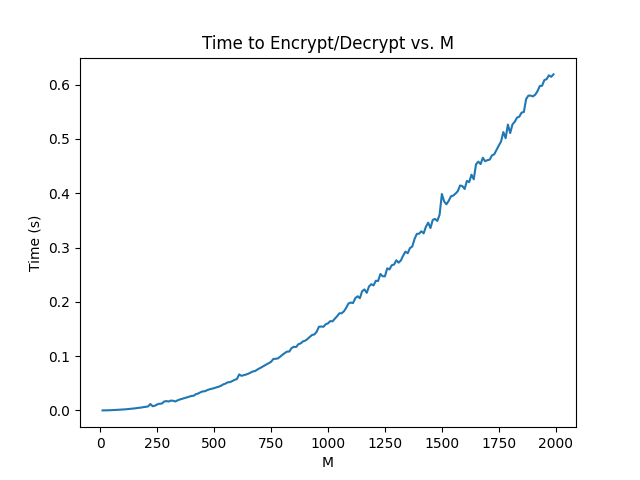
\includegraphics[width=0.4\textwidth]{../src/graphs/time_vs_m.png}
         &
        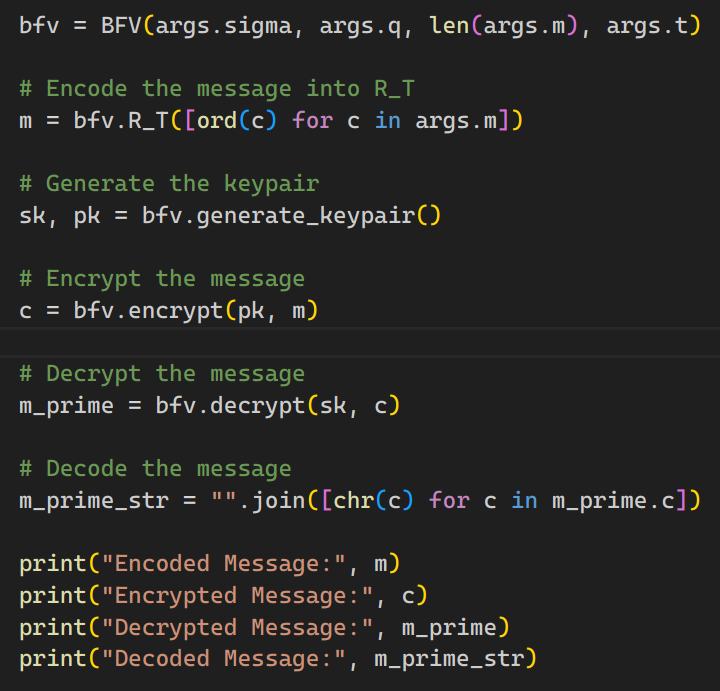
\includegraphics[width=0.30\textwidth]{../src/graphs/code_sample.png}
    \end{tabular}

    \caption{Left: Encryption time as a function of message length $m$. Right: Code sample of using my custom BFV class for encryption and decryption.}
    \label{fig:encryption-time}
\end{figure}

% Add bibliography

\printbibliography

\end{document}